\cchapter{Opening and rendering files}

TexMol reads molecule-specific PDB, PQR files (including simpler
XYZ, XYZR, PTS and a custom GOA formats), volume files (RAWIV, RAWV,
DX, MRC), surface files (RAW, RAWC, RAWN, RAWNC, OBJ, C2C) and a
custom NURBS file. By default, the data set is neither centered to
the view, nor rendered to screen. The user needs
to specifically render the data set after loading it.\\

\warning{If you do not have a good high end graphics card, or if it
is not set up properly to display using Cg, you will not see any
output on the screen. We are in the process of moving to OpenGL
Shading Language.}


\csection{Loading a molecule description file}

We support multiple molecular files. The most commonly used file
formats are PDB \cite{pdb} and PQR \cite{pqr}. We also have simple
file formats to describe general point sets: XYZ (list of centers on
successive lines), XYZR (same, includes radius next to center) and
PTS (similar to XYZ, but first line contains number of centers). The
properties box for molecular data sets is shown in figure
\ref{Figure:MoleculesPropertyBox}. There are two LODs as shown in
the figure, the color LOD and the object LOD.

\begin{figure}
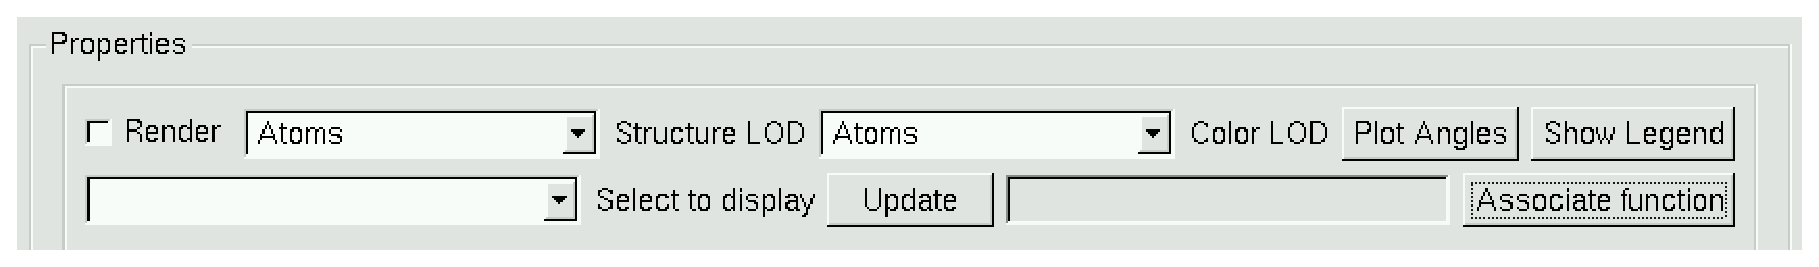
\includegraphics[width=5in]{Images/MoleculeFileProperties.ps}
\ccaption{The \emph{Properties widget} for molecule data sets allows
users to pick their choice of color and structure level of detail to
render. Other functions include associating a volumetric function
with the surfaces color.} \label{Figure:MoleculesPropertyBox}
\end{figure}

\subsection{The static hierarchy for biomolecules}

We use the biochemical hierarchy in our visualizations. For atoms,
we use the CPK model, with van der Waals radii. The colors and
radius used are described in the table in
\emph{elementInformation.h}. Atoms are grouped into residues, which
are approximated by spheres in the structure LOD. Secondary
structures are rendered with imposters like cylinders and helices.
Chains are rendered as a ball-and-stick model.

\begin{itemize}
\item Atoms. The atom sequence is the lowest, or finest level in the
hierarchy to obtain the primary structure of the molecule.

\item Residues. Atoms are grouped into their respective residues.

\item Secondary structures. Residues are grouped in to either
helices or sheets, or into dummy NULL structures.

\item Chains. The secondary structures are collected in to chains.
They form the tertiary structure.

\item Molecule. The highest or coarsest level in the static
hierarchy is the molecule itself.

\end{itemize}

After loading the molecule file, one can select a combination of
color and structure LOD to obtain various visualizations. To open a
PDB or PQR file, follow the steps shown in table
\ref{Table:OpenMoleculeFile}. A simple well known molecule to start
with would be hemoglobin (1A00.pdb), as it has multiple chains and
helices. Some interesting combinations of visualizations would be as
shown in figure \ref{Figure:hemoglobinVisualizations}. Table
\ref{Table:showHelices} explains how one can visualize the helices
in the loaded molecule.

\begin{figure}
     \centering
     \subfigure[Atoms colored with element colors]{
          \label{Figure:hemoglobinVisualizationsa}
          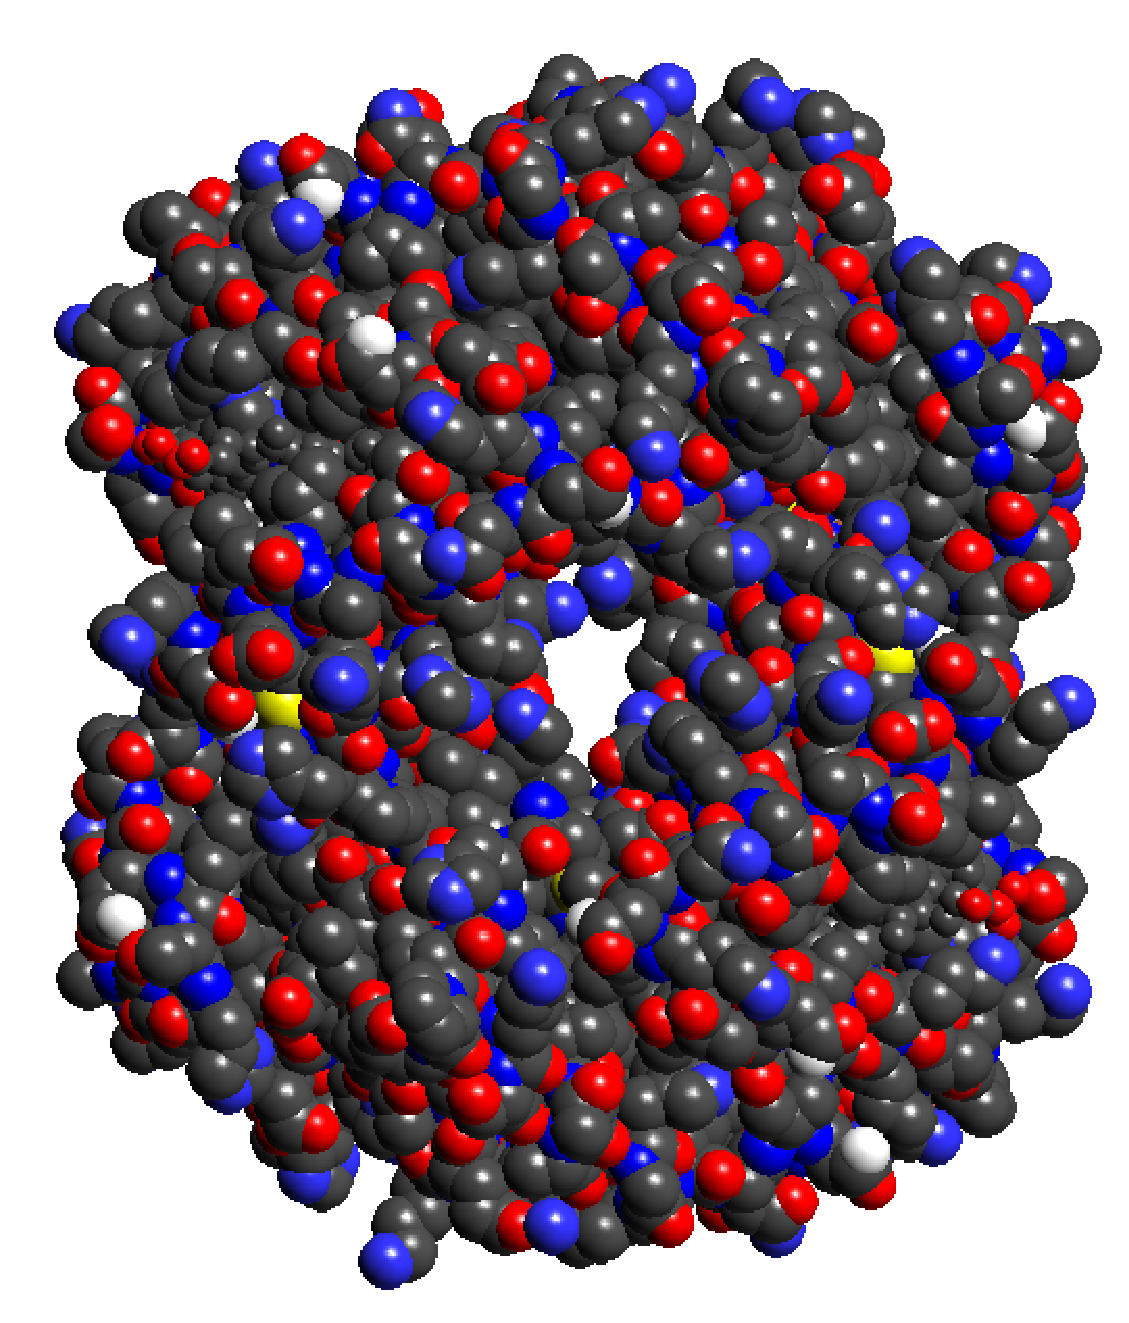
\includegraphics[width=.45\textwidth]{Images/Hemoglobin_Atoms.ps}}
     \hspace{.3in}
     \subfigure[Atoms colored with their respective residues colors]{
          \label{Figure:hemoglobinVisualizationsb}
          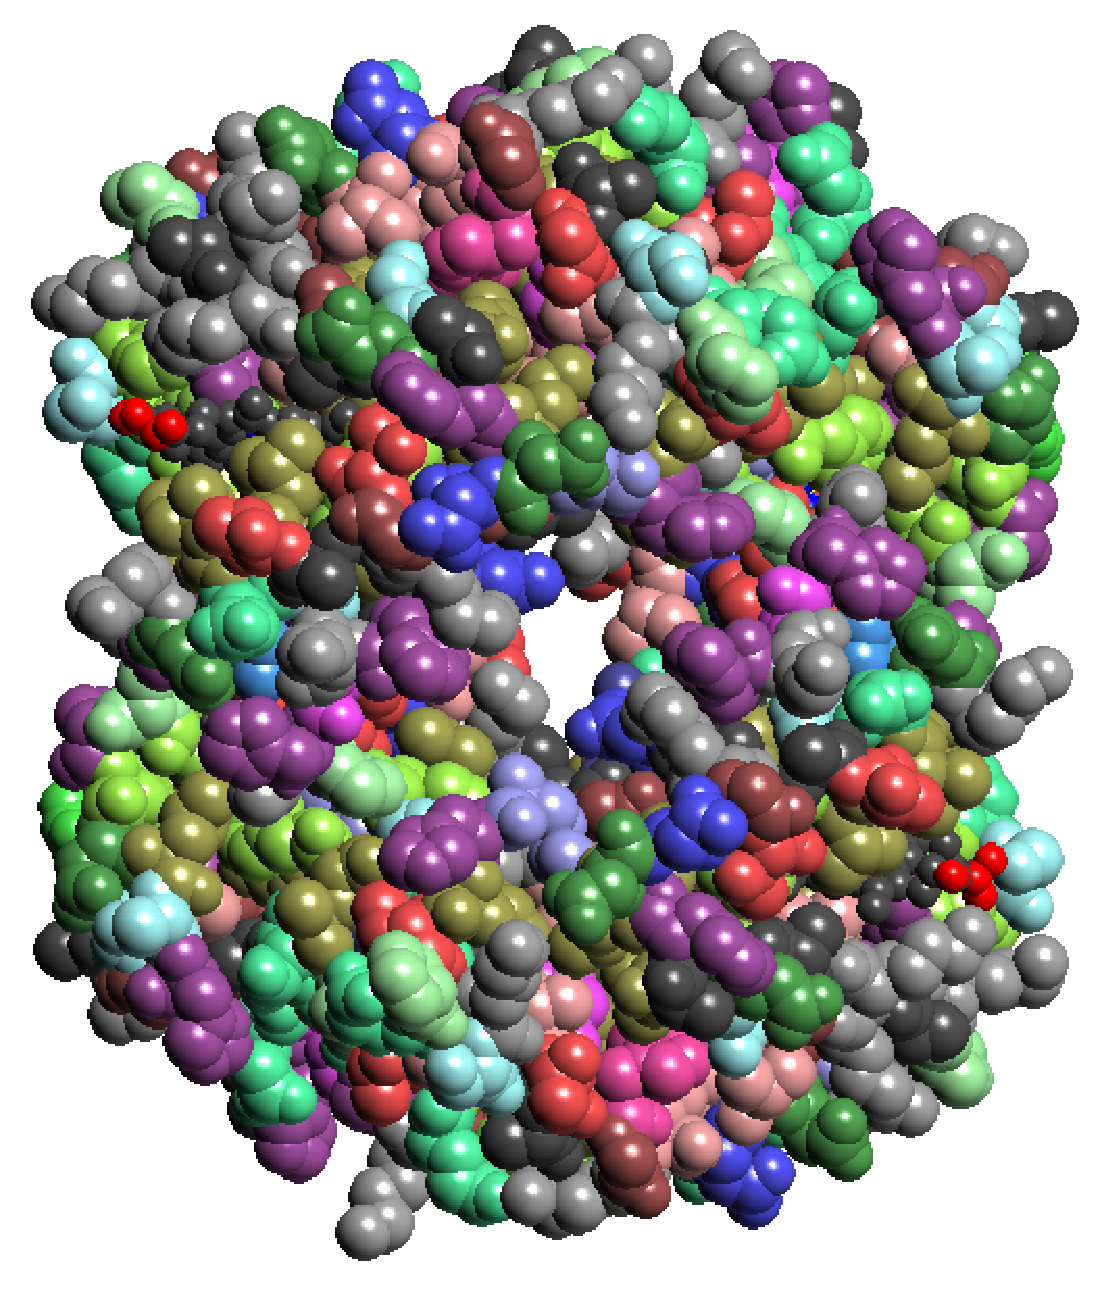
\includegraphics[width=.45\textwidth]{Images/Hemoglobin_atoms_residue_colors.ps}}\\
     \vspace{.3in}
     \subfigure[A coarser model with residues rendered as spheres]{
          \label{Figure:hemoglobinVisualizationsc}
          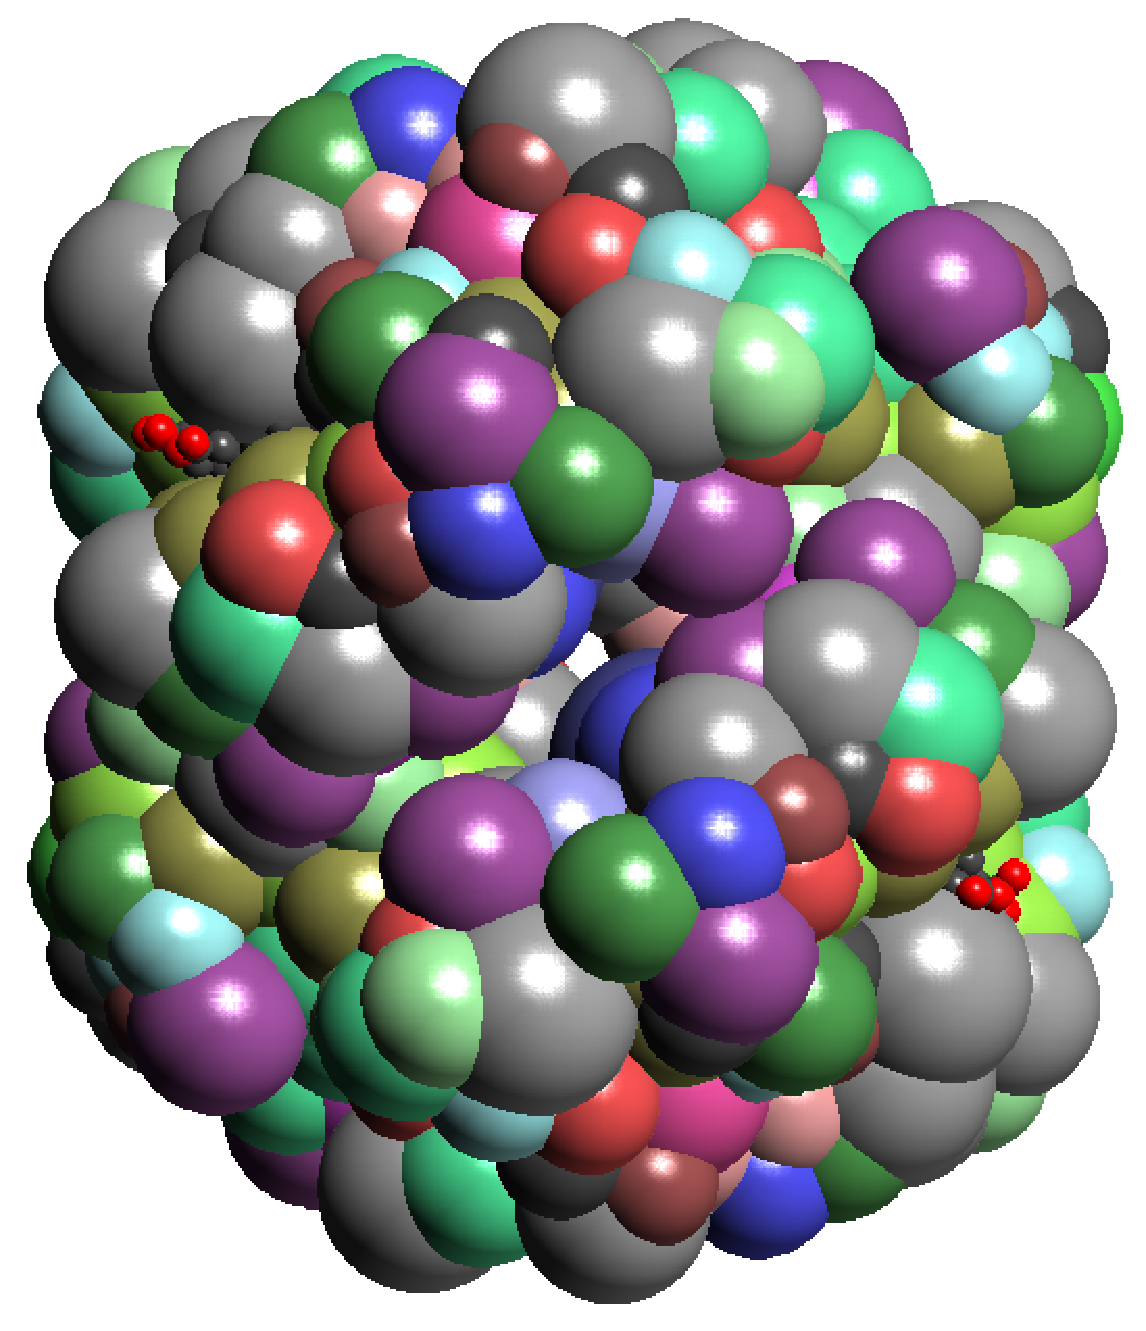
\includegraphics[width=.45\textwidth]{Images/Hemoglobin_Residues.ps}}
     \hspace{.3in}
     \subfigure[Helices forming the secondary structures in the molecule]{
          \label{Figure:hemoglobinVisualizationsd}
          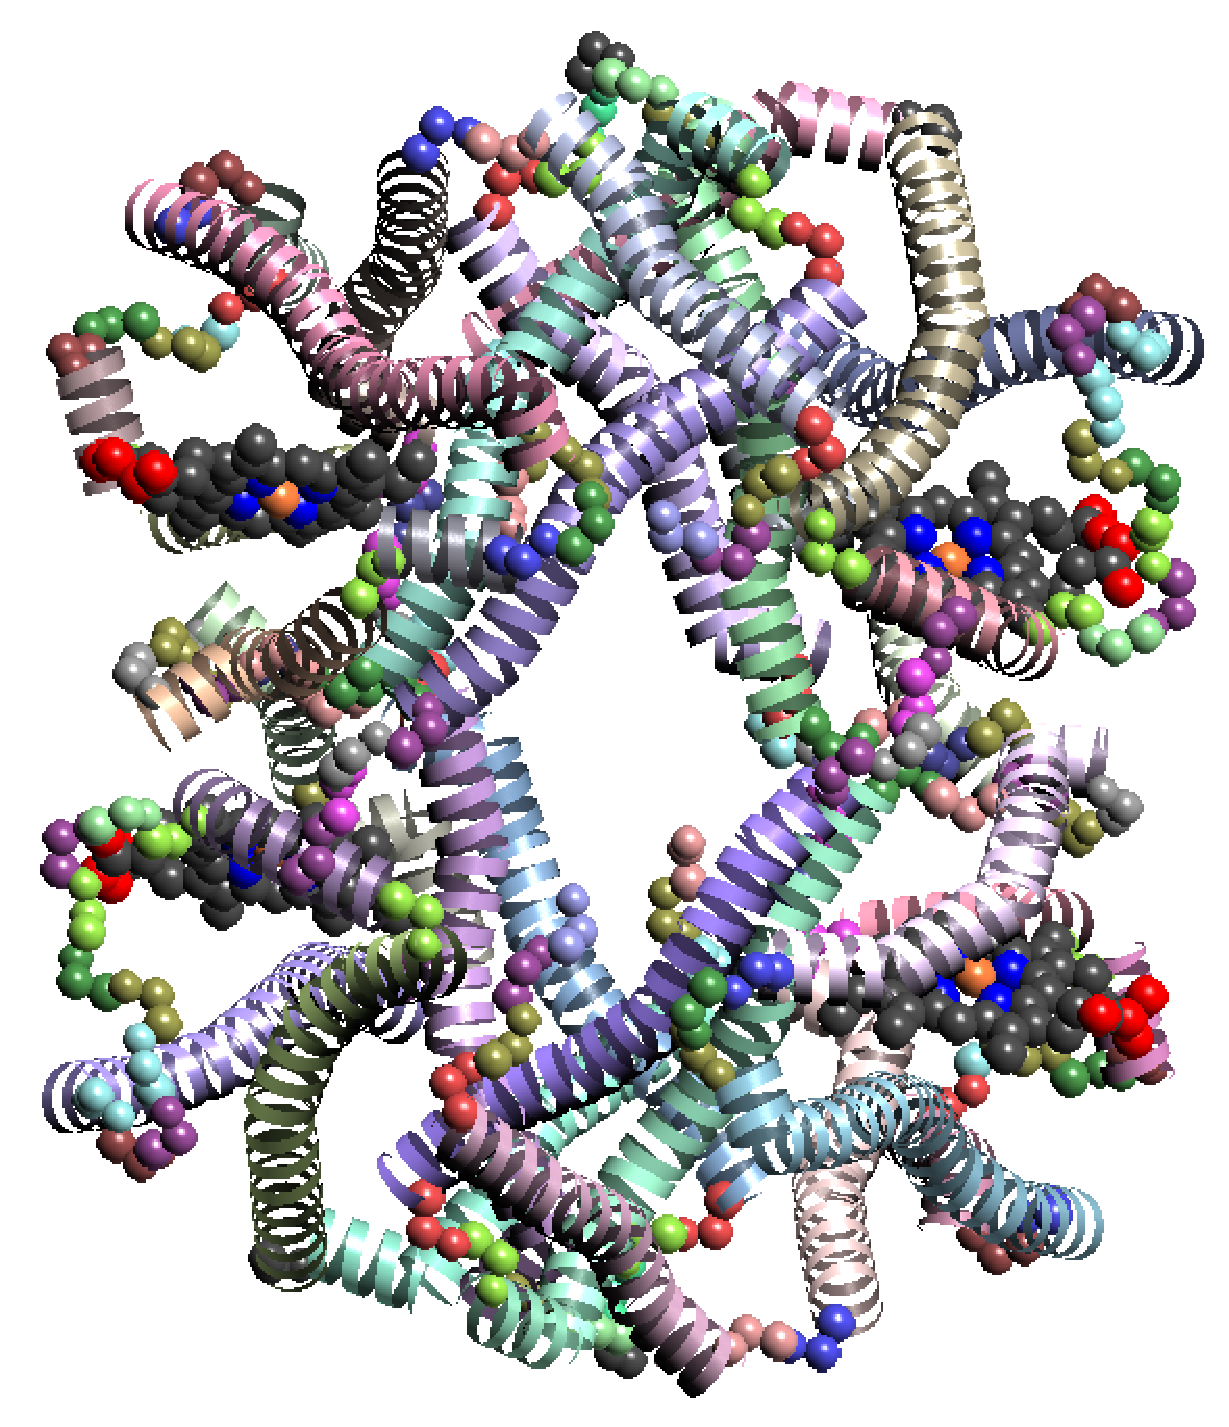
\includegraphics[width=.45\textwidth]{Images/Hemoglobin_ss.ps}}\\
     \caption{Molecules can be rendered at different color and structure level of details.
     Here we show the hemoglobin molecule (1A00.pdb) rendered in 4 different styles.}
     \label{Figure:hemoglobinVisualizations}
\end{figure}

\steps{Loading a molecule}{Table:OpenMoleculeFile}{ \item Select
File - Open from menu bar.
\item Choose a file name by pressing the File button and select a
PDB or PQR file.
\item If you know that you are choosing a isosahedral virus, check the isVirus check box.
\item Press OK to load the file, or Cancel to cancel this action.}

\steps{Visualizing helices in a molecule}{Table:showHelices}{\item
If you have not loaded a molecule, do so by following the steps
outlined in Table \ref{Table:OpenMoleculeFile}. \item Set the
Structure LOD to Secondary structures and the Color LOD to any item.
\item Render the molecule by checking the Render check box. \item If
the molecule is not visible in the current view point, you may need
to zoom out and translate to bring it in to view.}

\csection{Loading volume files}

We currently support four volume files including the scalar RAWIV,
MRC and DX formats, and vector valued RAWV formats. They are both
binary and ascii files and support multiple data types and sizes.
For a complete description, see the file format descriptions on the
CCV web site. To load volume files, follow the same steps as
outlined in table \ref{Table:OpenMoleculeFile}, but select a volume
file instead of a molecule file.

To render volume files and isosurfaces, you need to get familiar
with a widget called a color table, which is user interface for
reading a transfer map. A detailed description for the color table
can be found in the volume rover software user guide.

\csection{Loading surface files}

\warning{Surface files currently supported can be compressed or not.
The uncompressed files can take up to a few minutes to load for very
large meshes.}

 Like volume files, surface files do not need to deal with
molecules. \TexMol currently supports uncompressed (RAW, RAWC, RAWN,
RAWNC and OBJ) and compressed (c2c) surface files. To load any of
these file formats, table \ref{Table:OpenMoleculeFile} can be
followed with the right input file types. Both wireframe and surface
rendering modes are supported. The user can also view both together.
A visualization of the Mache molecule, showing the gorge is shown in
figure \ref{Figure:MACHE}. The OBJ file format is from Alias
Wavefront.

\begin{figure}
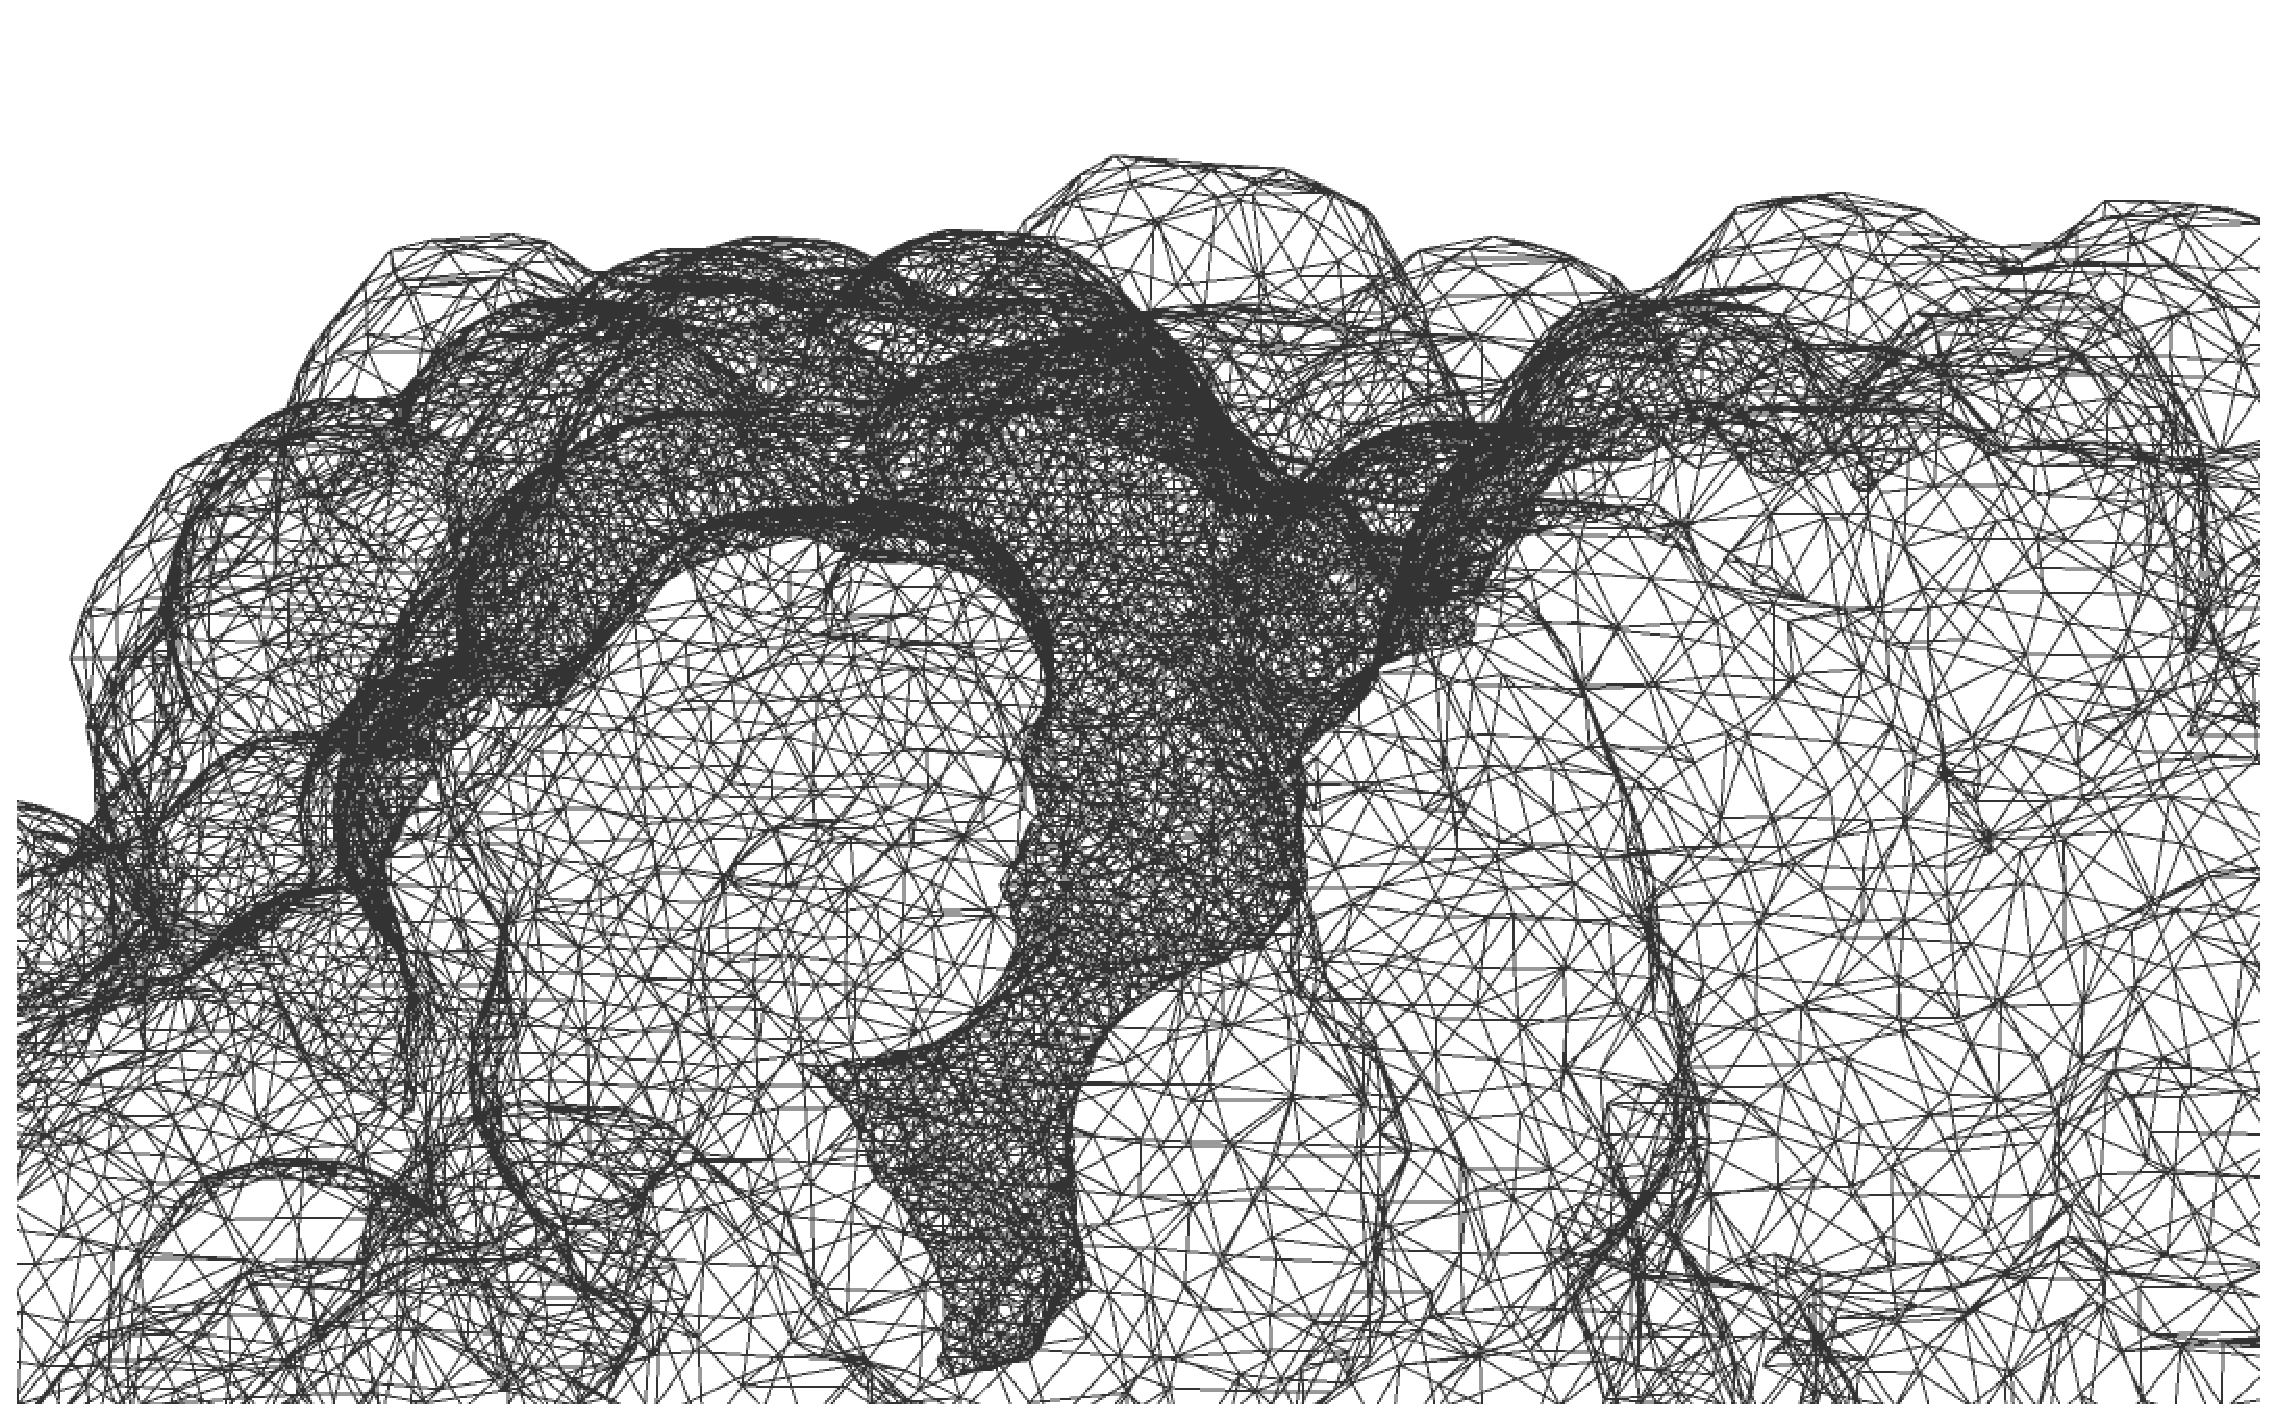
\includegraphics[width=5in]{Images/MacheWireframe.ps}
\ccaption{Wireframe rendering of a mesh, showing a gorge type
feature in the surface of the MACHE molecule.} \label{Figure:MACHE}
\end{figure}
